\documentclass{beamer}
\usepackage[utf8]{inputenc}
\usepackage[UKenglish]{babel}
\usepackage[UKenglish]{isodate}
\usepackage{tikz}
\usepackage[style=authoryear]{biblatex}
\usepackage{complexity}
\usepackage[vlined]{algorithm2e}
\usepackage{spot}
\usepackage{appendixnumberbeamer}

\usetikzlibrary{arrows.meta}
\usetikzlibrary{tikzmark}
\usetikzlibrary{positioning}
\tikzstyle{every picture}+=[remember picture]
\tikzstyle{na} = [baseline=-.5ex]

\beamertemplatenavigationsymbolsempty
\usetheme{Madrid}
\usecolortheme{seahorse}
\addbibresource{talk.bib}
\DeclareMathOperator{\leftlsquigarrow}{\text{\reflectbox{$\rightsquigarrow$}}}

\definecolor{c1}{HTML}{1b9e77}
\definecolor{c2}{HTML}{d95f02}
\definecolor{c3}{HTML}{7570b3}
\definecolor{c4}{HTML}{e7298a}

\newcommand{\one}{\textcolor{c1}{x_1}}
\newcommand{\two}{\textcolor{c2}{x_2}}
\newcommand{\three}{\textcolor{c3}{x_3}}
\newcommand{\four}{\textcolor{c4}{x_4}}
\newcommand{\highlight}[1]{%
  \colorbox{red!10}{$#1$}}

\author{Paulius Dilkas}
\title{Generating Random WMC Instances}
\subtitle{An Empirical Analysis with Varying Primal Treewidth}
\institute[NUS]{National University of Singapore, Singapore}
\date{CPAIOR 2023}
% 20 min talk

\begin{document}

\begin{frame}[noframenumbering,plain]
  \tikz[remember picture,overlay]{
    \node at ([yshift=20pt,xshift=-20pt]current page.south)
    {
\includegraphics[height=40pt]{nus.jpg}};
    \node at ([yshift=25pt,xshift=30pt]current page.south)
    {
\includegraphics[height=40pt]{inf.png}};
    \node at ([yshift=25pt,xshift=75pt]current page.south)
    {
\includegraphics[height=40pt]{ecr.jpg}};
    \node at ([yshift=20pt,xshift=140pt]current page.south)
    {
\includegraphics[height=20pt]{epsrc.png}};
  }
  \titlepage
\end{frame}

\begin{frame}{Which Algorithm Is Better? It Depends on the Data}
  \begin{center}
    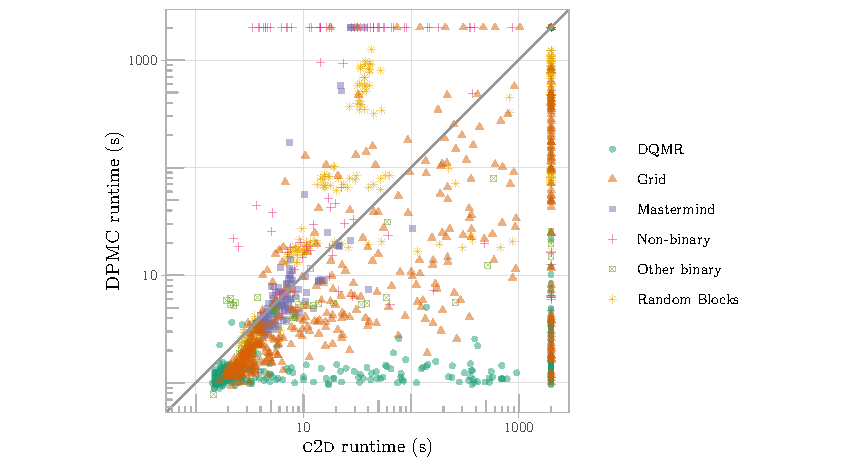
\includegraphics[width=\linewidth]{scatter}
  \end{center}

  The runtime data is from \textcolor{gray}{\textcite{DBLP:conf/sat/DilkasB21}}:
  various Bayesian networks encoded using the approach by
  \textcolor{gray}{\textcite{DBLP:conf/kr/Darwiche02}}
\end{frame}

\begin{frame}{The Problem: Weighted Model Counting (WMC)}
  \begin{columns}
    \begin{column}{0.5\textwidth}
      \begin{itemize}
        \item A generalisation of propositional model counting ($\#\SAT{}$)
        \item Applications:
        \begin{itemize}
          \item graphical models
          \item probabilistic programming
          \item neuro-symbolic AI
        \end{itemize}
        \item WMC algorithms use:
        \begin{itemize}
          \item dynamic programming
          \item knowledge compilation
          \item \SAT{} solvers
        \end{itemize}
      \end{itemize}
    \end{column}
    \begin{column}{0.5\textwidth}
      \begin{example}
        $w(x) = 0.3$, $w(\neg x) = 0.7$, $w(y) = 0.2$, $w(\neg y) = 0.8$
        \vspace{1cm}

        $\mathsf{WMC}(\alert{x \lor y}) = w(x)w(y) + w(x)w(\neg y) + w(\neg x)w(y) = 0.44$
      \end{example}
    \end{column}
  \end{columns}
\end{frame}

\begin{frame}{(Some of the) WMC Algorithms}
  \begin{itemize}
    \item \textsc{Cachet} \textcolor{gray}{\parencite{DBLP:conf/sat/SangBBKP04}}
          \begin{itemize}
            \item a SAT solver with \alert{clause learning} and \alert{component
                  caching}
          \end{itemize}
    \item \textsc{c2d} \textcolor{gray}{\parencite{DBLP:conf/ecai/Darwiche04}}
          \begin{itemize}
            \item knowledge compilation to \alert{d-DNNF}
          \end{itemize}
    \item \textsc{d4} \textcolor{gray}{\parencite{DBLP:conf/ijcai/LagniezM17}}
          \begin{itemize}
            \item knowledge compilation to \alert{decision-DNNF}
          \end{itemize}
    \item \textsc{miniC2D} \textcolor{gray}{\parencite{DBLP:conf/ijcai/OztokD15}}
          \begin{itemize}
            \item knowledge compilation to \alert{decision sentential decision
                  diagrams}
          \end{itemize}
    \item \textsc{DPMC} \textcolor{gray}{\parencite{DBLP:conf/cp/DudekPV20}}
          \begin{itemize}
            \item dynamic programming with \alert{algebraic decision diagrams}
                  and \alert{tree decomposition} based planning
          \end{itemize}
  \end{itemize}
\end{frame}

\begin{frame}{Tree Decompositions and Primal Treewidth}
  Formula in CNF:
  \[
    \phi = (\four{} \lor \neg \three{} \lor \one{}) \land (\neg \two{} \lor \four{}) \land (\neg \one{} \lor \two{} \lor \four{})
  \]
  \pause
  \begin{columns}
    \begin{column}{0.5\textwidth}
      Its primal graph:

      \hspace{1cm}
      \begin{tikzpicture}
        \node (one) at (0, 1) {$\one{}$};
        \node (two) at (1, 1) {$\two{}$};
        \node (three) at (0, 0) {$\three{}$};
        \node (four) at (1, 0) {$\four{}$};
        \draw (one) -- (two);
        \draw (one) -- (three);
        \draw (one) -- (four);
        \draw (two) -- (four);
        \draw (three) -- (four);
      \end{tikzpicture}
    \end{column}
    \begin{column}{0.5\textwidth}
      \pause
      Its minimum-width tree decomposition:

      \begin{tikzpicture}[every text node part/.style={align=center}]
        \node[circle,draw] (one) {$\one{}$ $\two{}$\\$\four{}$};
        \node[circle,draw,right=of one] (two) {$\one{}$ $\three{}$\\$\four{}$};
        \draw (one) -- (two);
      \end{tikzpicture}
    \end{column}
  \end{columns}
  \centering
  \vfill
  \pause
  $\therefore$ the primal treewidth of \structure{$\phi$} is \structure{2}
\end{frame}

\begin{frame}{The Parameterised Complexity of WMC Algorithms}
  Let \structure{$n$} be the number of \structure{variables} and \structure{$m$} be
  the number of \structure{clauses}.
  \begin{itemize}
    \item Component caching (used in \textsc{Cachet}) is
          \alert{$2^{\mathcal{O}(w)}n^{\mathcal{O}(1)}$}, where \structure{$w$}
          is the \structure{branchwidth} of the underlying hypergraph
          \textcolor{gray}{\parencite{DBLP:journals/jair/BacchusDP09}}
          \begin{itemize}
            \item Branchwidth is within a constant factor of primal treewidth
          \end{itemize}
    \item \textsc{c2d} is based on an algorithm, which is
          \alert{$\mathcal{O}(2^{w}mw)$}, where \structure{$w$} is at most
          \structure{primal treewidth}
          \textcolor{gray}{\parencite{DBLP:journals/jacm/Darwiche01,DBLP:conf/ecai/Darwiche04}}
    \item \textsc{DPMC} can be shown to be \alert{$\mathcal{O}(4^{w}mn)$}, where
          \structure{$w$} is an upper bound on \structure{primal treewidth}
  \end{itemize}
\end{frame}

\begin{frame}{From Random SAT to Random WMC}
  We introduce parameter \structure{$\rho \in [0, 1]$} that biases the
  probability distribution towards adding variables that would introduce fewer
  new edges to the primal graph.

  \vfill
  \begin{columns}[t]
    \begin{column}{0.5\linewidth}
      Example partially-filled formula:
      \structure{$(\neg x_{5} \lor x_{2} \lor x_{1}) \land (x_{5} \lor \alert{\mathord{?}} \lor \mathord{?})$}
    \end{column}
    \begin{column}{0.4\linewidth}
      Its primal graph:

      \begin{tikzpicture}
        \node (a) at (0.5, 1) {$x_{1}$};
        \node (b) at (0, 0) {$x_{2}$};
        \node (c) at (1, 0) {\spot{$x_{5}$}};
        \node (d) at (2, 1) {$x_{3}$};
        \node (e) at (2, 0) {$x_{4}$};
        \draw (a) -- (b);
        \draw[blue,thick] (b) -- (c);
        \draw[blue,thick] (c) -- (a);
        \draw (current bounding box.north east) rectangle (current bounding box.south west);
      \end{tikzpicture}
    \end{column}
  \end{columns}

  \begin{block}{The probability distribution for the next variable}
    Base probability of each variable being chosen:
    \[
      \frac{1 - \rho}{4}.
    \]

    Both \structure{$x_{1}$} and \structure{$x_{2}$} get a bonus probability of
    \structure{$\rho/2$} for each being the endpoint of \alert{one} out of
    the \alert{two} neighbourhood edges.
  \end{block}
\end{frame}

\begin{frame}{The Relationship Between \alert{$\rho$} and Primal Treewidth}
  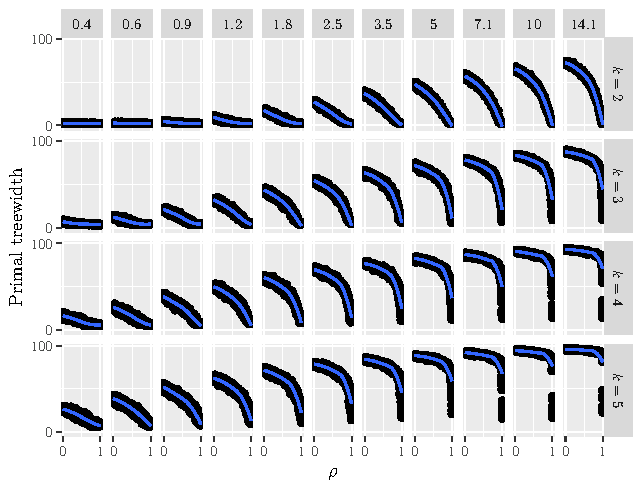
\includegraphics{regular_repetitiveness.pdf}
\end{frame}
% NOTE: density (i.e., ratio of clauses and variables) at the top

% NOTE: from now on, we're only looking at 3-CNF formulas. Maybe introduce a
% slide for that (+ numbers of variables, etc.)?

\begin{frame}{Peak Hardness w.r.t. Density}
  Let \structure{$\mu$} denote the \alert{density}, i.e., the number of clauses
  divided by the number of variables.
  \begin{itemize}
    \item \textsc{Cachet} is known to peak at \structure{$\mu = 1.8$}
          \textcolor{gray}{\parencite{DBLP:conf/sat/SangBBKP04}}
    \item \textcolor{gray}{\textcite{DBLP:conf/aaai/Pehoushek00}} show some
          $\#\SAT{}$ algorithms to peak at \structure{$\mu = 1.2$} and
          \structure{$\mu = 1.9$}
          \pause
    \item In our experiments:
    \begin{itemize}
      \item \textsc{DPMC} peaks at \structure{$\mu = 2.2$}
      \item all other algorithms peak at \structure{$\mu = 1.9$}
    \end{itemize}
  \end{itemize}
\end{frame}

\begin{frame}{Peak Hardness w.r.t. Density (when $\rho = 0$)}
  \centering
  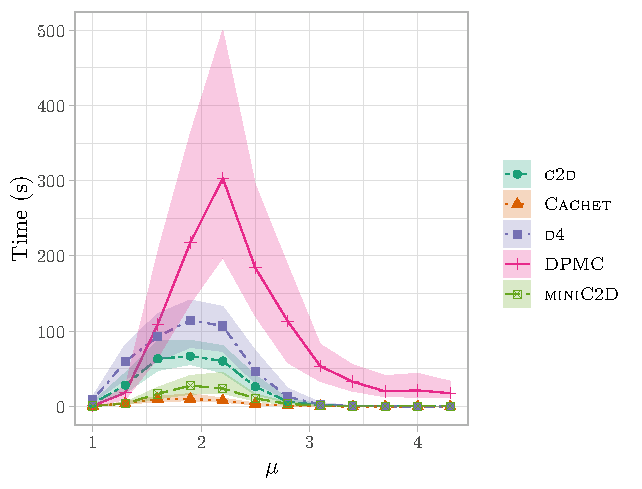
\includegraphics{treewidth.pdf}
\end{frame}

\begin{frame}{Hardness w.r.t. Primal Treewidth (when $\mu = 1.9$)}
  \centering
  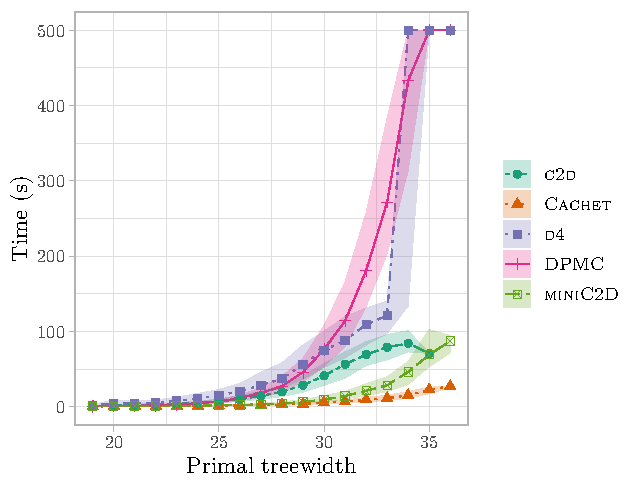
\includegraphics{treewidth2.pdf}
\end{frame}

\begin{frame}{Is The Relationship Exponential?}
  Let us fit the model \structure{$\ln t \sim \alpha w + \beta$}, i.e.,
  \structure{$t \sim e^{\beta}{(e^{\alpha})}^{w}$}, where \structure{$t$} is
  \alert{runtime}, and \structure{$w$} is \alert{primal treewidth}
  \begin{overprint}%
  \only<2>{\centerline{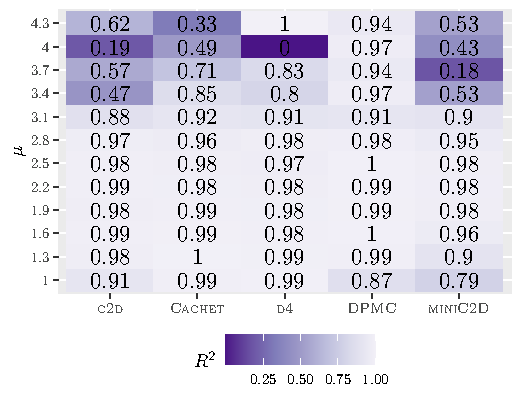
\includegraphics{r2.pdf}}}%
  \uncover<3>{\centerline{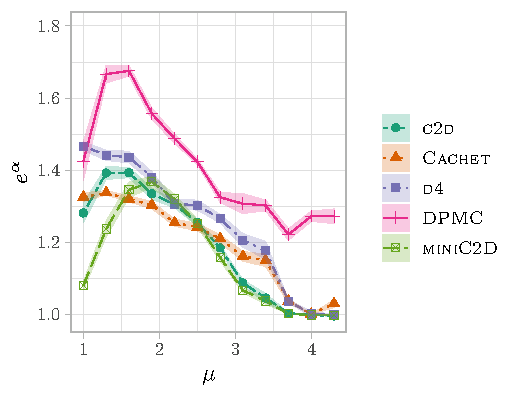
\includegraphics{linearbase.pdf}}}%
  \end{overprint}
\end{frame}

\begin{frame}{Does Real Data Confirm Our Observations?}
  \centering
  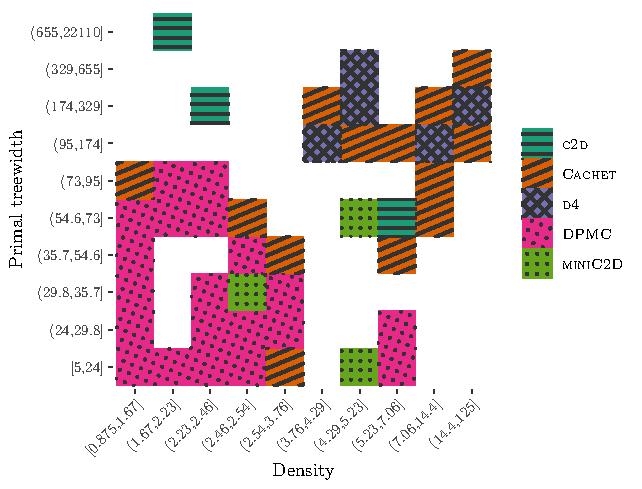
\includegraphics{real}
\end{frame}

\begin{frame}{Bonus: How \textsc{DPMC} Reacts to Redundancy in Weights}
  Let \structure{$\epsilon$} be the proportion of variables \structure{$x$} s.t.
  \structure{$w(x) = w(\neg x) = 0.5$}

  \centering
  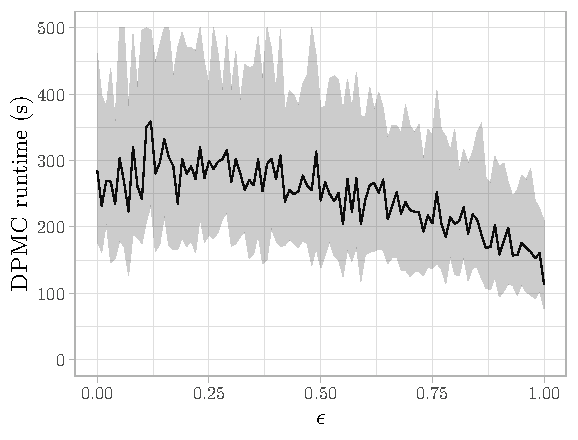
\includegraphics{epsilon}
\end{frame}

\begin{frame}{Summary}
  \begin{itemize}
    \item This work introduced a \alert{random model} for WMC instances with a
          parameter that indirectly controls \alert{primal treewidth}
    \item Observations:
    \begin{itemize}
      \item All algorithms \alert{scale exponentially} w.r.t.\ primal treewidth
      \item The running time of \textsc{DPMC}:
      \begin{itemize}
        \item peaks at a higher density
        \item and scales worse w.r.t.\ primal treewidth
      \end{itemize}
    \end{itemize}
    \item Future work:
    \begin{itemize}
      \item A theoretical relationship between \structure{$\rho$} and primal treewidth
      \item Non-\structure{$k$}-CNF instances
      \item Algorithm portfolios for WMC
    \end{itemize}
  \end{itemize}
\end{frame}

\appendix

\begin{frame}{Generating Random WMC Instances: The Algorithm}
  \begin{columns}
    \begin{column}{0.69\textwidth}
      \begin{algorithm}[H]
        \SetKwData{kcnf}{kcnf}
        \SetKwFunction{NewVariable}{newVariable}
        $\structure{\phi} \gets \text{empty CNF formula}$\;
        $\structure{G} \gets \text{empty graph}$\;
        \For{$i \gets 1$ \KwTo \alert{$m$\tikz[na] \node[coordinate] (m1) {};}}{
          $\structure{X} \gets \emptyset$\;
          \For{$j \gets 1$ \KwTo \alert{$k$\tikz[na] \node[coordinate] (k1) {};}}{
            $\structure{x} \gets \alert{\NewVariable{$X$, $G$}}\tikz[na] \node[coordinate] (f1) {};$\;
            $\mathcal{V}(\structure{G}) \gets \mathcal{V}(\structure{G}) \cup \{\, \structure{x} \,\}$\;
            $\mathcal{E}(\structure{G}) \gets \mathcal{E}(\structure{G}) \cup \{\, \{\,\structure{x}, \structure{y}\,\} \mid \structure{y} \in \structure{X} \,\}$\;
            $\structure{X} \gets \structure{X} \cup \{\, \structure{x} \,\}$\;
          }
          $\structure{\phi} \gets \structure{\phi} \cup \{\,\{\, \structure{l} \leftlsquigarrow \mathcal{U}\{\, \structure{x}, \neg \structure{x} \,\} \mid \structure{x} \in \structure{X} \,\}\,\}$\tikz[na] \node[coordinate] (c1) {};\;
        }
      \end{algorithm}
    \end{column}
    \begin{column}{0.31\textwidth}
      \begin{itemize}
        \item\tikz[na] \node[coordinate] (m2) {};the number of clauses
        \item\tikz[na] \node[coordinate] (k2) {};clause width
        \item\tikz[na] \node[coordinate] (f2) {};a function to pick a variable
        \item\tikz[na] \node[coordinate] (c2) {};a (fair) coin flip
      \end{itemize}
    \end{column}
  \end{columns}
  \begin{tikzpicture}[overlay]
    \path[-Latex,shorten >=0.6cm,shorten <=0.5cm,dashed] (m2) edge (m1);
    \path[-Latex,shorten >=0.6cm,shorten <=0.5cm,dashed] (k2) edge (k1);
    \path[-Latex,shorten >=0.1cm,shorten <=0.5cm,dashed] (f2) edge (f1);
    \path[-Latex,shorten >=0.1cm,shorten <=0.5cm,dashed] ([shift={(0, 0.2)}]c2) edge (c1);
  \end{tikzpicture}
\end{frame}

\begin{frame}{How to Pick a Variable}
  Parameter \structure{$\rho \in [0, 1]$} biases the probability distribution
  towards adding variables that would introduce fewer new edges.

  \begin{algorithm}[H]
    \SetKwProg{Fn}{Function}{:}{}
    \Fn{\NewVariable{set of variables \structure{$X$}, primal graph \structure{$G$}}}{
      $\structure{N} \gets \{\, \structure{e} \in \mathcal{E}(\structure{G}) \mid |\structure{e} \cap \structure{X}| = 1 \,\}$\;
      \lIf{$\structure{N} = \emptyset$}{\Return{$\structure{x} \leftlsquigarrow \mathcal{U}(\{\, \structure{x_1}, \structure{x_2}, \dots, \structure{x_{\alert{n}}} \,\} \setminus \structure{X})$}}
      \Return{$\structure{x} \leftlsquigarrow \left(\{\, \structure{x_1}, \structure{x_2}, \dots, \structure{x}_{\alert{n}} \,\} \setminus \structure{X}, \structure{y} \mapsto \highlight{\frac{1 - \alert{\rho}}{\alert{n} - |\structure{X}|} + \alert{\rho}\frac{|\{\, \structure{z} \in X \mid \{\,\structure{y}, \structure{z}\,\} \in \mathcal{E}(\structure{G}) \,\}|}{|\structure{N}|}}\right)$}\;
    }
  \end{algorithm}
\end{frame}

\end{document}
